\documentclass[]{article}
\usepackage{graphicx}

%opening
\title{CPSC425 A2}
\author{Eric Semeniuc - 54383161}

\begin{document}

\maketitle


\textbf{1-3:}
\begin{verbatim}
>>> main.demoShowPyramid()
>>> 
\end{verbatim}

\begin{figure}[ht]
	\centering
	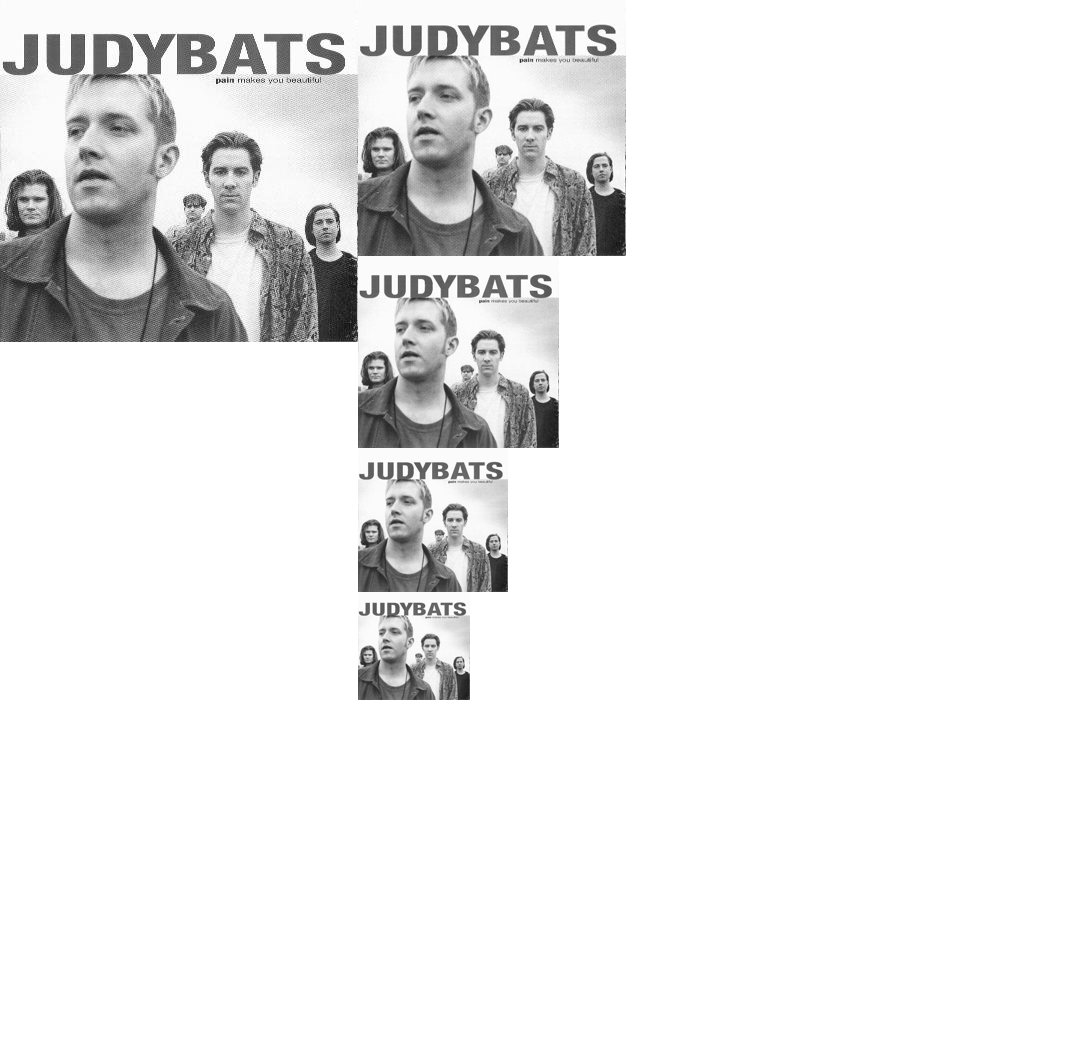
\includegraphics{pyramid.png}
	\label{fig:pyramid}
\end{figure}


\textbf{1-5:}
Threshold = 0.586\\

\begin{figure}[ht]
\centering
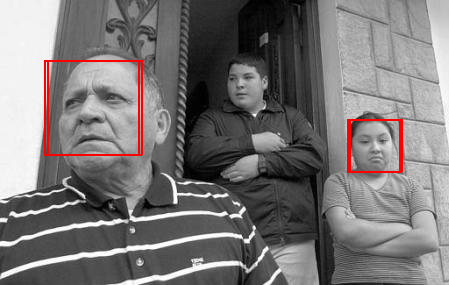
\includegraphics{fam.png}
\label{fig:fam}
\end{figure}

\begin{figure}[ht]
	\centering
	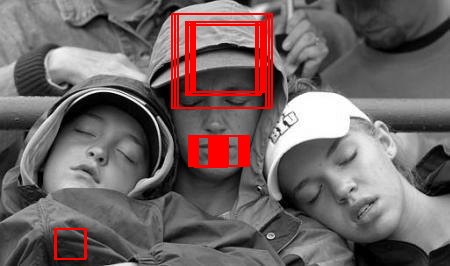
\includegraphics{fans.png}
	\label{fig:fans}
\end{figure}
\begin{figure}[ht]
	\centering
	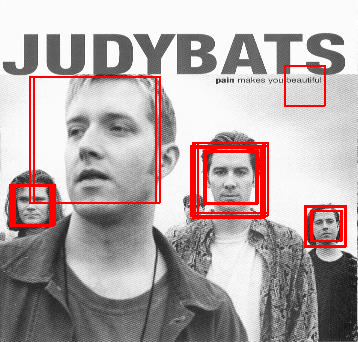
\includegraphics{judy.png}
	\label{fig:judy}
\end{figure}
\begin{figure}[ht]
	\centering
	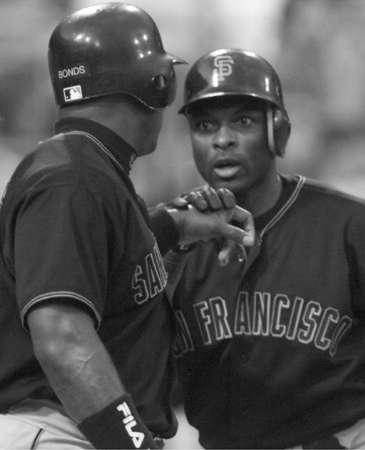
\includegraphics{sports.png}
	\label{fig:sports}
\end{figure}
\begin{figure}[ht]
	\centering
	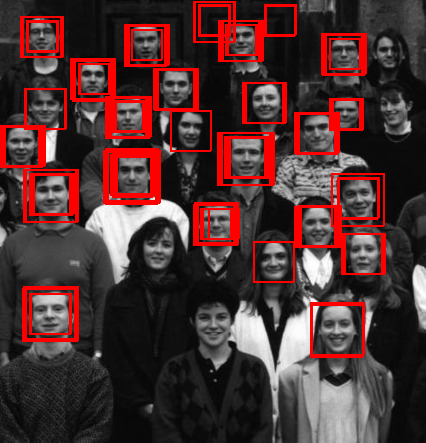
\includegraphics{students.png}
	\label{fig:students}
\end{figure}
\begin{figure}[ht]
	\centering
	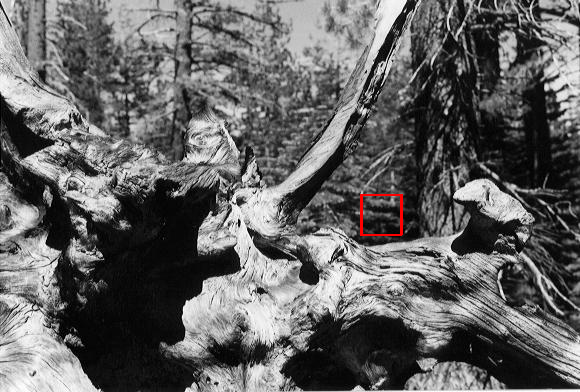
\includegraphics{tree.png}
	\label{fig:tree}
\end{figure}


\textbf{Missed}
\begin{verbatim}
family: 1
fans: 3
judy: 1
sport: 1
student: 4
tree: 0
total = 10
\end{verbatim}

\textbf{False Positives}
\begin{verbatim}
family: 0
fans: 6
judy: 1
sport: 0
student: 3
tree: 1
total = 11
\end{verbatim}

\textbf{1-6:}\\
\textbf{Recall Rate}
\begin{verbatim}
family: 2/3
fans: 0/3
judy: 4/5
sport: 0/1
student: 23/27
tree: 0/0
\end{verbatim}
``fans" has low recall rate as there are either hoods which cause a dark silhouette around the face or hats, and the eyes are closed. In addition, 2 of the faces are not facing straight, so the template will match poorly.\\

``sport" has low recall rate as the face is of a man of African descent, which is unlike the template, which has a
face of Caucasian descent. Since there is so much difference in the brightness level, the face will not be matched by the template.\\

``tree" is a degenerate case as there are no faces, and division by 0 is undefined

In general NCC is not rotationally invariant, adaptive to different brightness levels, or robust to partial occlusion. The above examples demonstrate the flaws of NCC.


\end{document}
